
\section{Impulse Resonse Function}

The impluse response of the economy to a one grid point nominal shock is shown in Figs~\ref{irf1} and \ref{irf2}. The IRF on impact is 98.5\% in this economy (as a fraction of the nominal shock). The IRF dies out in eight to ten periods but it takes a couple of months for the small variations to die out completely.
\begin{figure}[H]
    \centering
    \begin{minipage}{0.48\textwidth}
        \centering
        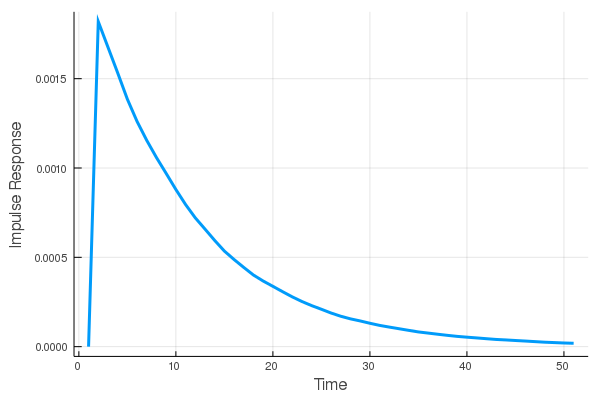
\includegraphics[width = \textwidth]{../tasks/Golosov_lucas/output/C_irf_50_periods.png}
        \caption{IRF till 50 periods after the shock}
        \label{irf1}
    \end{minipage}
    \begin{minipage}{0.48\textwidth}
        \centering
        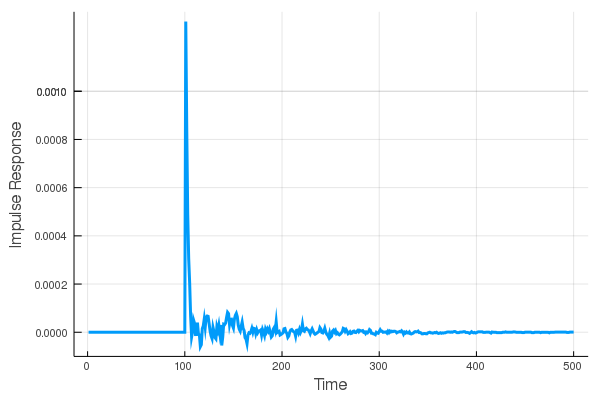
\includegraphics[width=\textwidth]{../tasks/Golosov_lucas/output/C_irf_500_periods.png}
        \caption{IRF for the entire simulation}
        \label{irf2}
    \end{minipage}
\end{figure}

The variance of the output in the baseline economy is . When we double the menu cost from 0.045 to 0.09 the variance of the output increases by 3.038 times.
On doubling the menu cost from 0.045 to 0.09 the variance of output increase by 3.038 times.

\section{Hazard}

The Hazard Function of the economy is as expected from the theory. The firms essentially follow a sS rule and adjust only when the price gaps get more than a certain thresholds. The probability of adjustment is zero within this interval and then jumps immediately to one outside this boundary.
\begin{figure}[H]
    \centering
    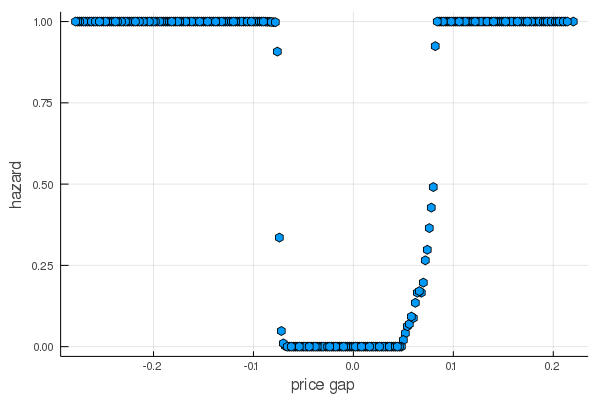
\includegraphics[width = 0.6\textwidth]{../tasks/Golosov_lucas/output/hazard_gl.png}
    \caption{Hazard}
    \label{}
\end{figure}

\section{Price Change Distribution}

Once the firm's price gap gets beyond the inaction interval, they immediately adjust to the optimal. However, due to the presence of aggregate shocks we do not get just the two mass points in the case of standard golosov lucas. Rather we get the distribution as in Fig~\ref{pcgl}.
\begin{figure}[H]
    \centering
    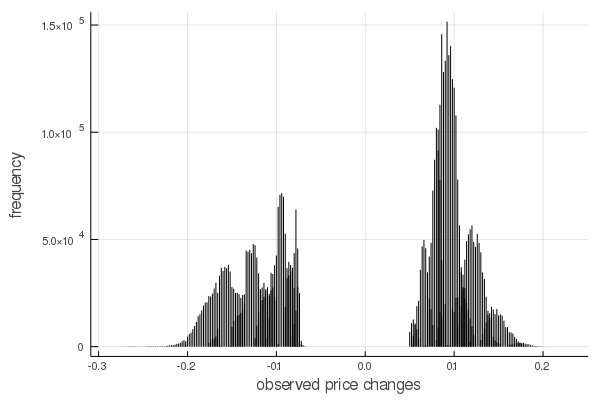
\includegraphics[width = 0.6\textwidth]{../tasks/Golosov_lucas/output/observed_p_changes_gl.png}
    \caption{Observed Price Changes}
    \label{pcgl}
\end{figure}

\section{Ergodic Price Gap Distribution}

In the presence of a positive drift and aggregate shocks to nominal spending, we get the following distribution of the price gaps in the model.
\begin{figure}[H]
    \centering
    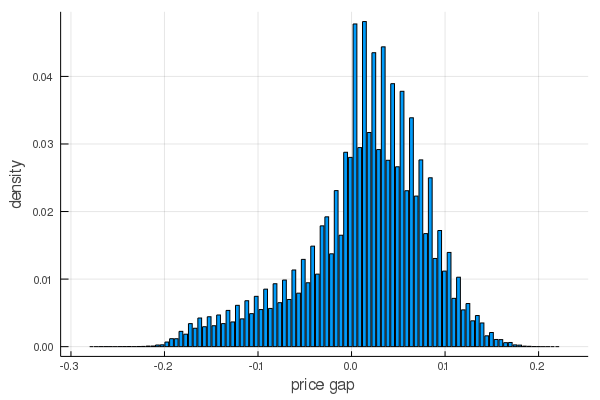
\includegraphics[width = 0.6\textwidth]{../tasks/Golosov_lucas/output/price_gap_dist.png}
    \caption{Price Gap Distribution}
    \label{}
\end{figure}
